Figure \ref{fig:precision_recall_curves} presents the precision-recall curves corresponding to Figures \ref{fig:discriminative_precision_recall} and \ref{fig:discriminative_precision_recall_relational}. Figure \ref{fig:tic_tac_toe_precision_recall_curce} corresponds to the panel in Figure \ref{fig:discriminative_precision_recall} and Figure \ref{fig:relational_precision_recall_curve} corresponds to the panel in Figure \ref{fig:discriminative_precision_recall_relational}. Note that these precision-recall curves have been obtained by varying the number of rules.

\begin{figure}[thb]
\begin{center}
\begin{subfigure}{.49\textwidth}
  \captionsetup{skip = 2pt}
  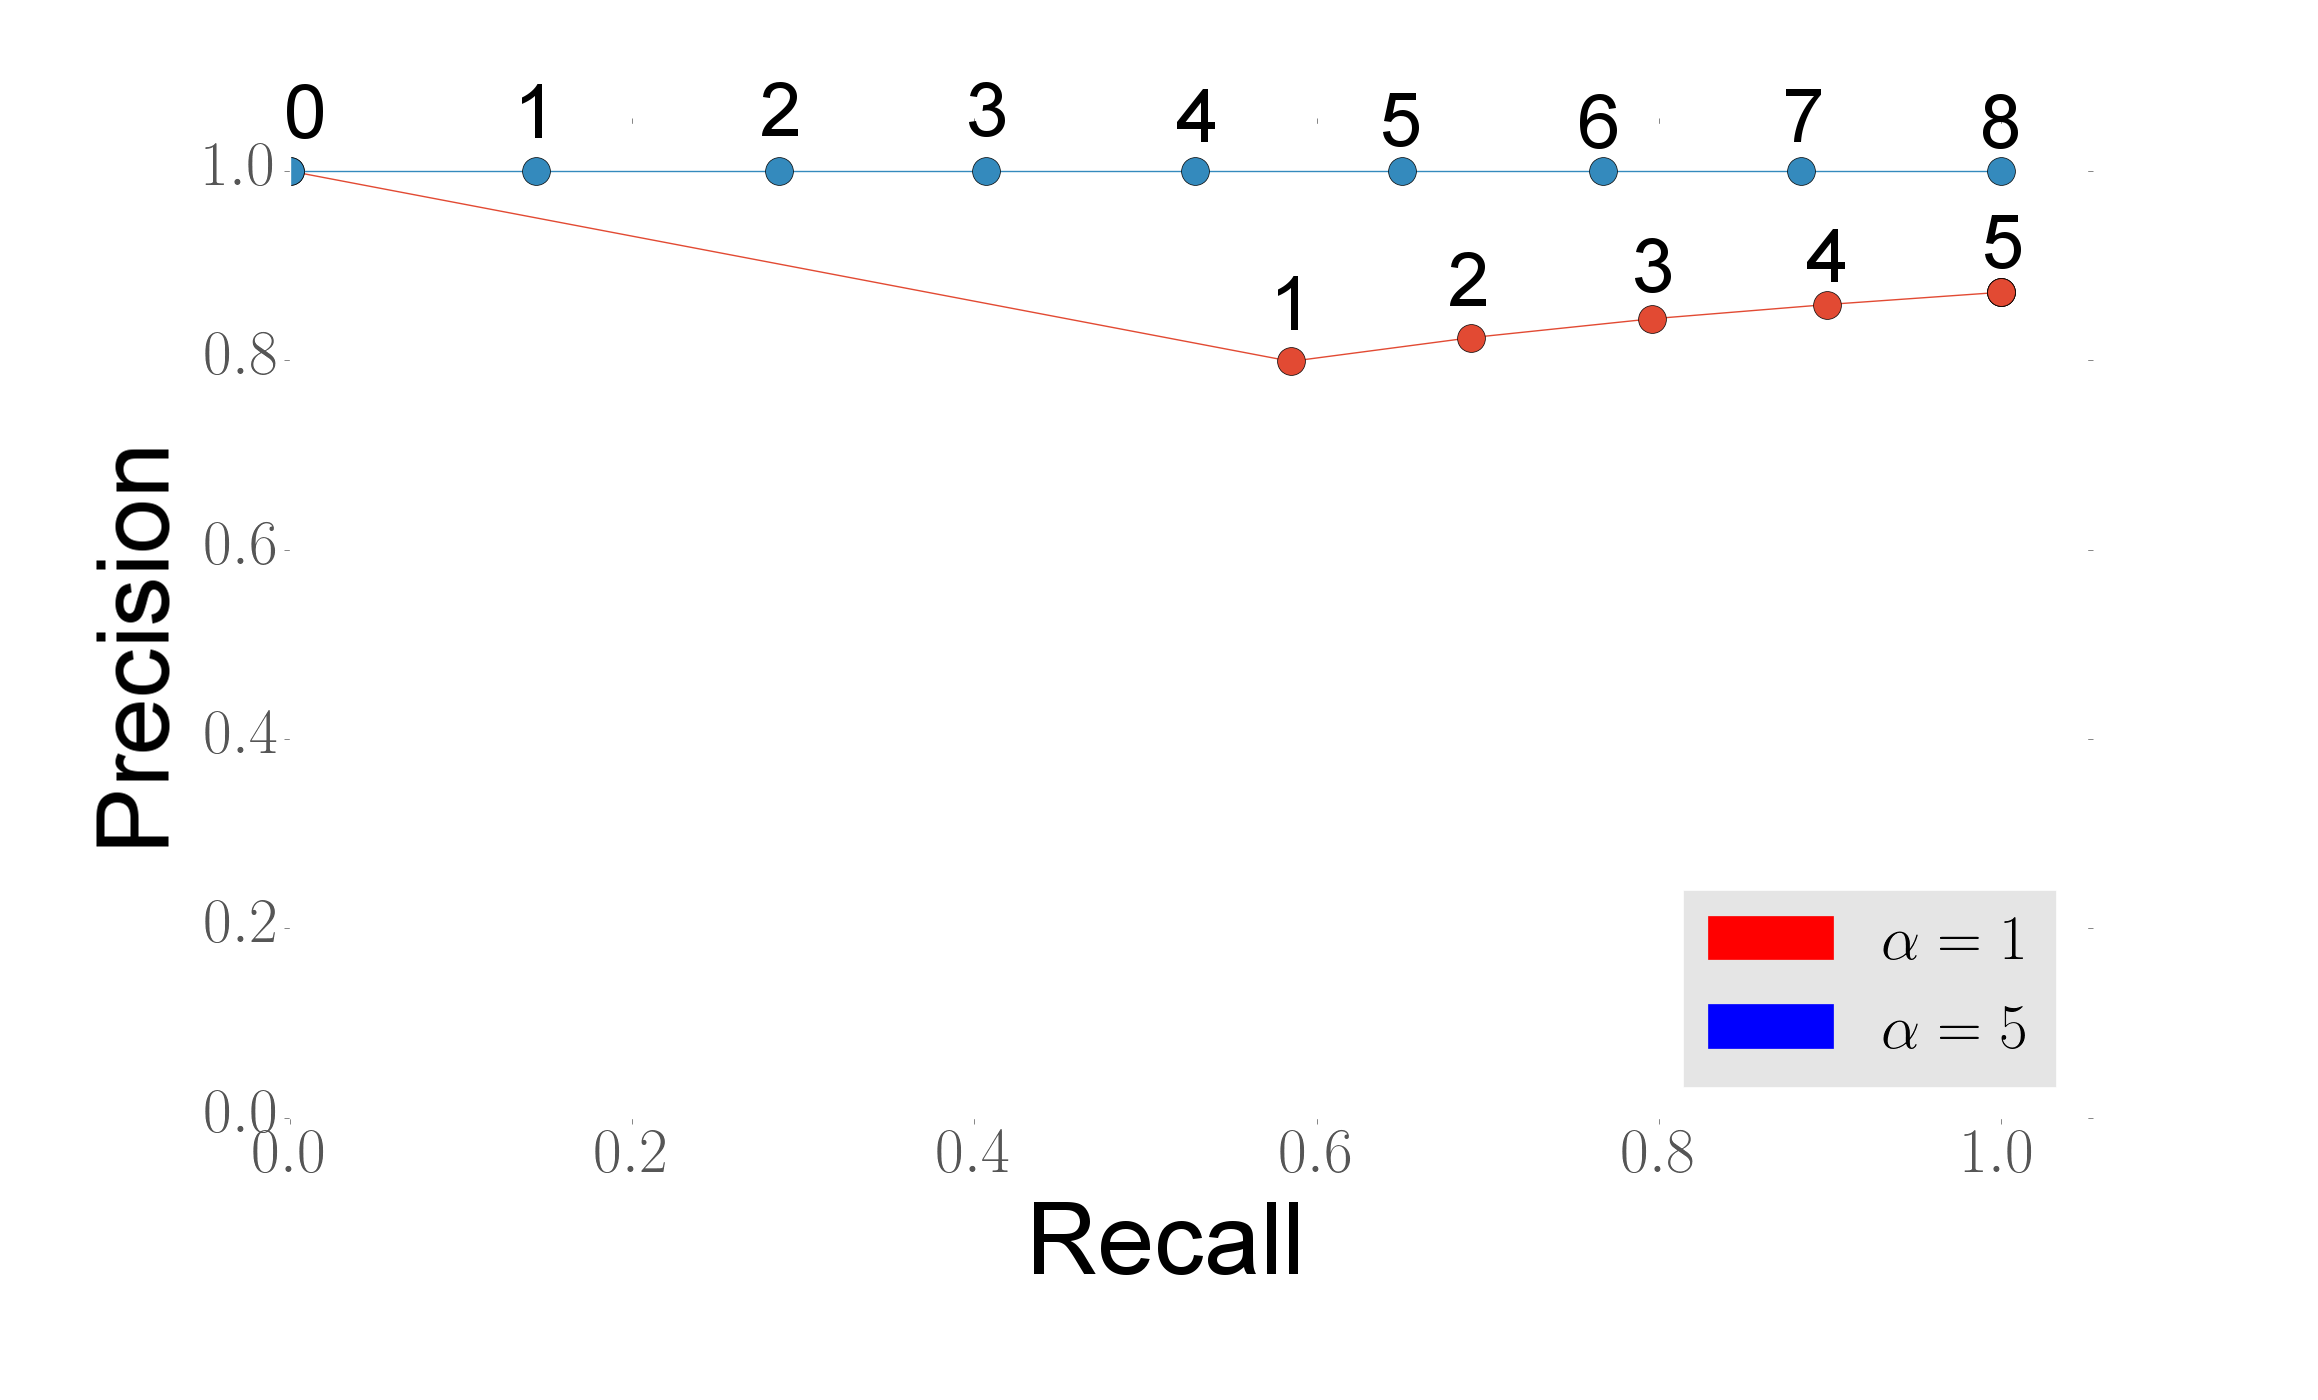
\includegraphics[width=\textwidth]{tic_tac_toe_precision_recall.png}
  \captionsetup{skip = -6pt}
  \caption{Tic-tac-toe discriminative pattern set mining}
  \label{fig:tic_tac_toe_precision_recall_curce}
\end{subfigure}
   \hfill 
\begin{subfigure}{.49\textwidth}
  \captionsetup{skip = 2pt}
  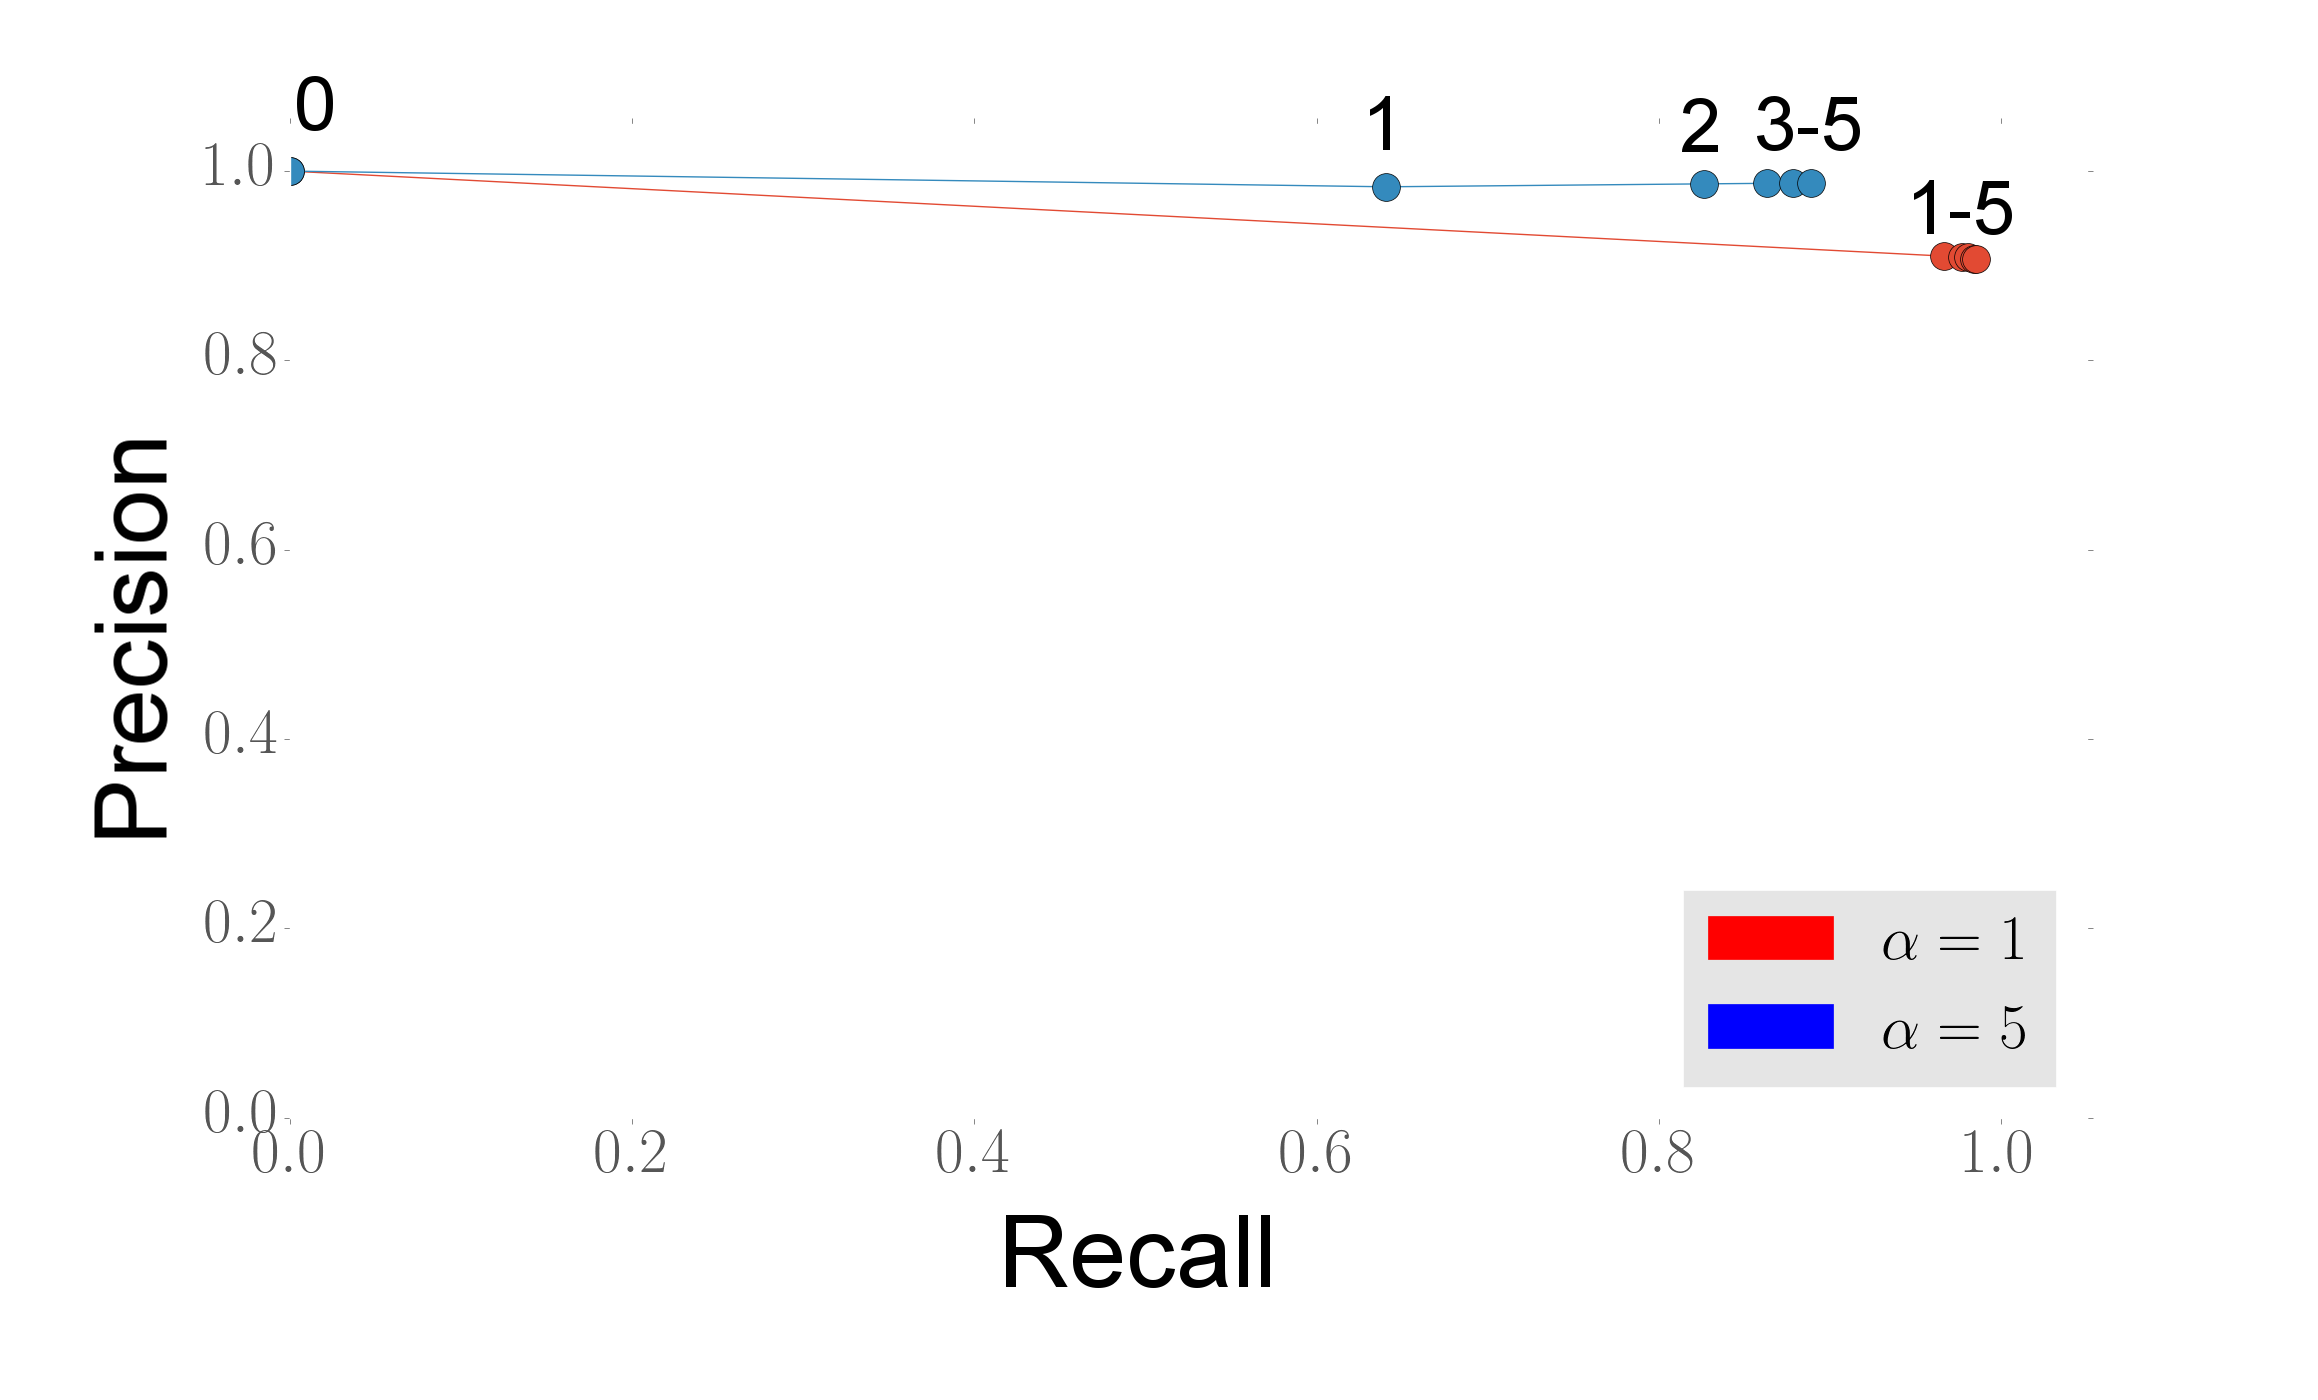
\includegraphics[width=\textwidth]{precision_recall_purely_relational.png}
  \captionsetup{skip = -6pt}
  \caption{Purely relational discriminative mining}
  \label{fig:relational_precision_recall_curve}
 \end{subfigure}
 \end{center}
  \captionsetup{skip = -6pt}
  \caption{Precision recall curves for discriminative learning for different $\alpha$, i.e., for two weights of covering negative atoms. For different number of learned rules, indicated on each point (starting from zero).}
  \label{fig:precision_recall_curves}
\end{figure}

